\documentclass{beamer}\usepackage[]{graphicx}\usepackage[]{color}
%% maxwidth is the original width if it is less than linewidth
%% otherwise use linewidth (to make sure the graphics do not exceed the margin)
\makeatletter
\def\maxwidth{ %
  \ifdim\Gin@nat@width>\linewidth
    \linewidth
  \else
    \Gin@nat@width
  \fi
}
\makeatother

\definecolor{fgcolor}{rgb}{0.196, 0.196, 0.196}
\newcommand{\hlnum}[1]{\textcolor[rgb]{0.063,0.58,0.627}{#1}}%
\newcommand{\hlstr}[1]{\textcolor[rgb]{0.063,0.58,0.627}{#1}}%
\newcommand{\hlcom}[1]{\textcolor[rgb]{0.588,0.588,0.588}{#1}}%
\newcommand{\hlopt}[1]{\textcolor[rgb]{0.196,0.196,0.196}{#1}}%
\newcommand{\hlstd}[1]{\textcolor[rgb]{0.196,0.196,0.196}{#1}}%
\newcommand{\hlkwa}[1]{\textcolor[rgb]{0.231,0.416,0.784}{#1}}%
\newcommand{\hlkwb}[1]{\textcolor[rgb]{0.627,0,0.314}{#1}}%
\newcommand{\hlkwc}[1]{\textcolor[rgb]{0,0.631,0.314}{#1}}%
\newcommand{\hlkwd}[1]{\textcolor[rgb]{0.78,0.227,0.412}{#1}}%
\let\hlipl\hlkwb

\usepackage{framed}
\makeatletter
\newenvironment{kframe}{%
 \def\at@end@of@kframe{}%
 \ifinner\ifhmode%
  \def\at@end@of@kframe{\end{minipage}}%
  \begin{minipage}{\columnwidth}%
 \fi\fi%
 \def\FrameCommand##1{\hskip\@totalleftmargin \hskip-\fboxsep
 \colorbox{shadecolor}{##1}\hskip-\fboxsep
     % There is no \\@totalrightmargin, so:
     \hskip-\linewidth \hskip-\@totalleftmargin \hskip\columnwidth}%
 \MakeFramed {\advance\hsize-\width
   \@totalleftmargin\z@ \linewidth\hsize
   \@setminipage}}%
 {\par\unskip\endMakeFramed%
 \at@end@of@kframe}
\makeatother

\definecolor{shadecolor}{rgb}{.97, .97, .97}
\definecolor{messagecolor}{rgb}{0, 0, 0}
\definecolor{warningcolor}{rgb}{1, 0, 1}
\definecolor{errorcolor}{rgb}{1, 0, 0}
\newenvironment{knitrout}{}{} % an empty environment to be redefined in TeX

\usepackage{alltt}

% load packages
\usepackage{tikz}
\usepackage{graphicx}
\usepackage{upquote}
\usepackage{listings}
\usepackage{hyperref}
\usepackage{color}
\usepackage{lmodern}



% define a bunch of colors
\definecolor{gray}{RGB}{110,110,110}
\definecolor{darkgray}{RGB}{100,100,100}
\definecolor{lightgray}{RGB}{200,200,200}
\definecolor{lightgrey}{RGB}{200,200,200}
\definecolor{turquoise}{RGB}{81,193,188}
\definecolor{mamey}{RGB}{255,107,107}
\definecolor{tomato}{RGB}{255,136,136}
\definecolor{mandarina}{RGB}{229,169,25}
\definecolor{lemon}{rgb}{0.81,0.95,0.29}
\definecolor{bluesky}{rgb}{0.71,0.81,0.96}
\definecolor{chiclamino}{RGB}{107,174,214}
\definecolor{violet}{RGB}{133,135,211}

\definecolor{foreground}{RGB}{81,141,193}
\definecolor{background}{RGB}{246,244,240}
\definecolor{highlight}{RGB}{229,169,25}
\definecolor{lowlight}{RGB}{200,200,200}

% setting beamer colors
\setbeamercolor{title}{fg=lightgray}
\setbeamercolor{frametitle}{fg=lightgray}
\setbeamercolor{block title}{fg=turquoise}
\setbeamercolor{structure}{fg=turquoise}
\setbeamercolor{titlelike}{fg=title}
\setbeamercolor{subtitle}{fg=turquoise}
\setbeamercolor{institute}{fg=gray}
\setbeamercolor{normal text}{fg=gray,bg=background}

\setbeamercolor{palette primary}{fg=lightgray}
\setbeamercolor{palette secondary}{fg=lightgray}
\setbeamercolor{palette tertiary}{fg=lightgray}

\setbeamerfont{itemize/enumerate subbody}{size=\footnotesize}
\setbeamerfont{itemize/enumerate subitem}{size=\footnotesize}

\hypersetup{
  colorlinks=true,
  urlcolor=tomato,
  linkcolor=lightgray
}

% commands
\newcommand{\code}[1]{\texttt{#1}}
\newcommand{\high}[1]{\textcolor{highlight}{#1}}
\newcommand{\low}[1]{\textcolor{lowlight}{#1}}
\newcommand{\highcode}[1]{\textcolor{highlight}{\texttt{#1}}}


%\usecolortheme{rose}
\setbeamertemplate{blocks}[rounded]
\setbeamertemplate{footline}[frame number] 
\setbeamertemplate{navigation symbols}{}
\setbeamertemplate{frametitle}[default][center]
\useoutertheme{infolines}  % add footlines
\setbeamersize{text margin left=25pt,text margin right=25pt}



% to remove empty brackets of \institution
\makeatletter
\setbeamertemplate{footline}
{
  \leavevmode%
  \hbox{%
  \begin{beamercolorbox}[wd=.333333\paperwidth,ht=2.25ex,dp=1ex,center]{author in head/foot}%
    \usebeamerfont{author in head/foot}\insertshortauthor%~~\beamer@ifempty{\insertshortinstitute}{}{(\insertshortinstitute)}
  \end{beamercolorbox}%
  \begin{beamercolorbox}[wd=.333333\paperwidth,ht=2.25ex,dp=1ex,center]{title in head/foot}%
    \usebeamerfont{title in head/foot}\insertshorttitle
  \end{beamercolorbox}%
  \begin{beamercolorbox}[wd=.333333\paperwidth,ht=2.25ex,dp=1ex,right]{date in head/foot}%
    \usebeamerfont{date in head/foot}\insertshortdate{}\hspace*{2em}
    \insertframenumber{} / \inserttotalframenumber\hspace*{2ex} 
  \end{beamercolorbox}}%
  \vskip0pt%
}
\makeatother



\title[Getting data from the web with R]{\LARGE Getting Data from the Web with R} 
\subtitle[Web Data in R]{\large Part 1: Introduction}
\author[gastonsanchez.com]{
 \textcolor{gray}{\textbf{G}aston \textbf{S}anchez}
}
\institute[]{\scriptsize \textcolor{lightgray}{April-May 2014}}
\date[CC BY-SA-NC 4.0]{
 \textcolor{lightgrey}{\tiny{Content licensed under 
 \href{http://creativecommons.org/licenses/by-nc-sa/4.0/}{CC BY-NC-SA 4.0}}}
}
\IfFileExists{upquote.sty}{\usepackage{upquote}}{}
\begin{document}




%--- the titlepage frame -------------------------%

\begin{frame}[plain]
 \titlepage
\end{frame}

%------------------------------------------------

{ % all template changes are local to this group.
    \setbeamertemplate{navigation symbols}{}
    \begin{frame}[plain]
        \begin{tikzpicture}[remember picture,overlay]
            \node[at=(current page.center)] {
                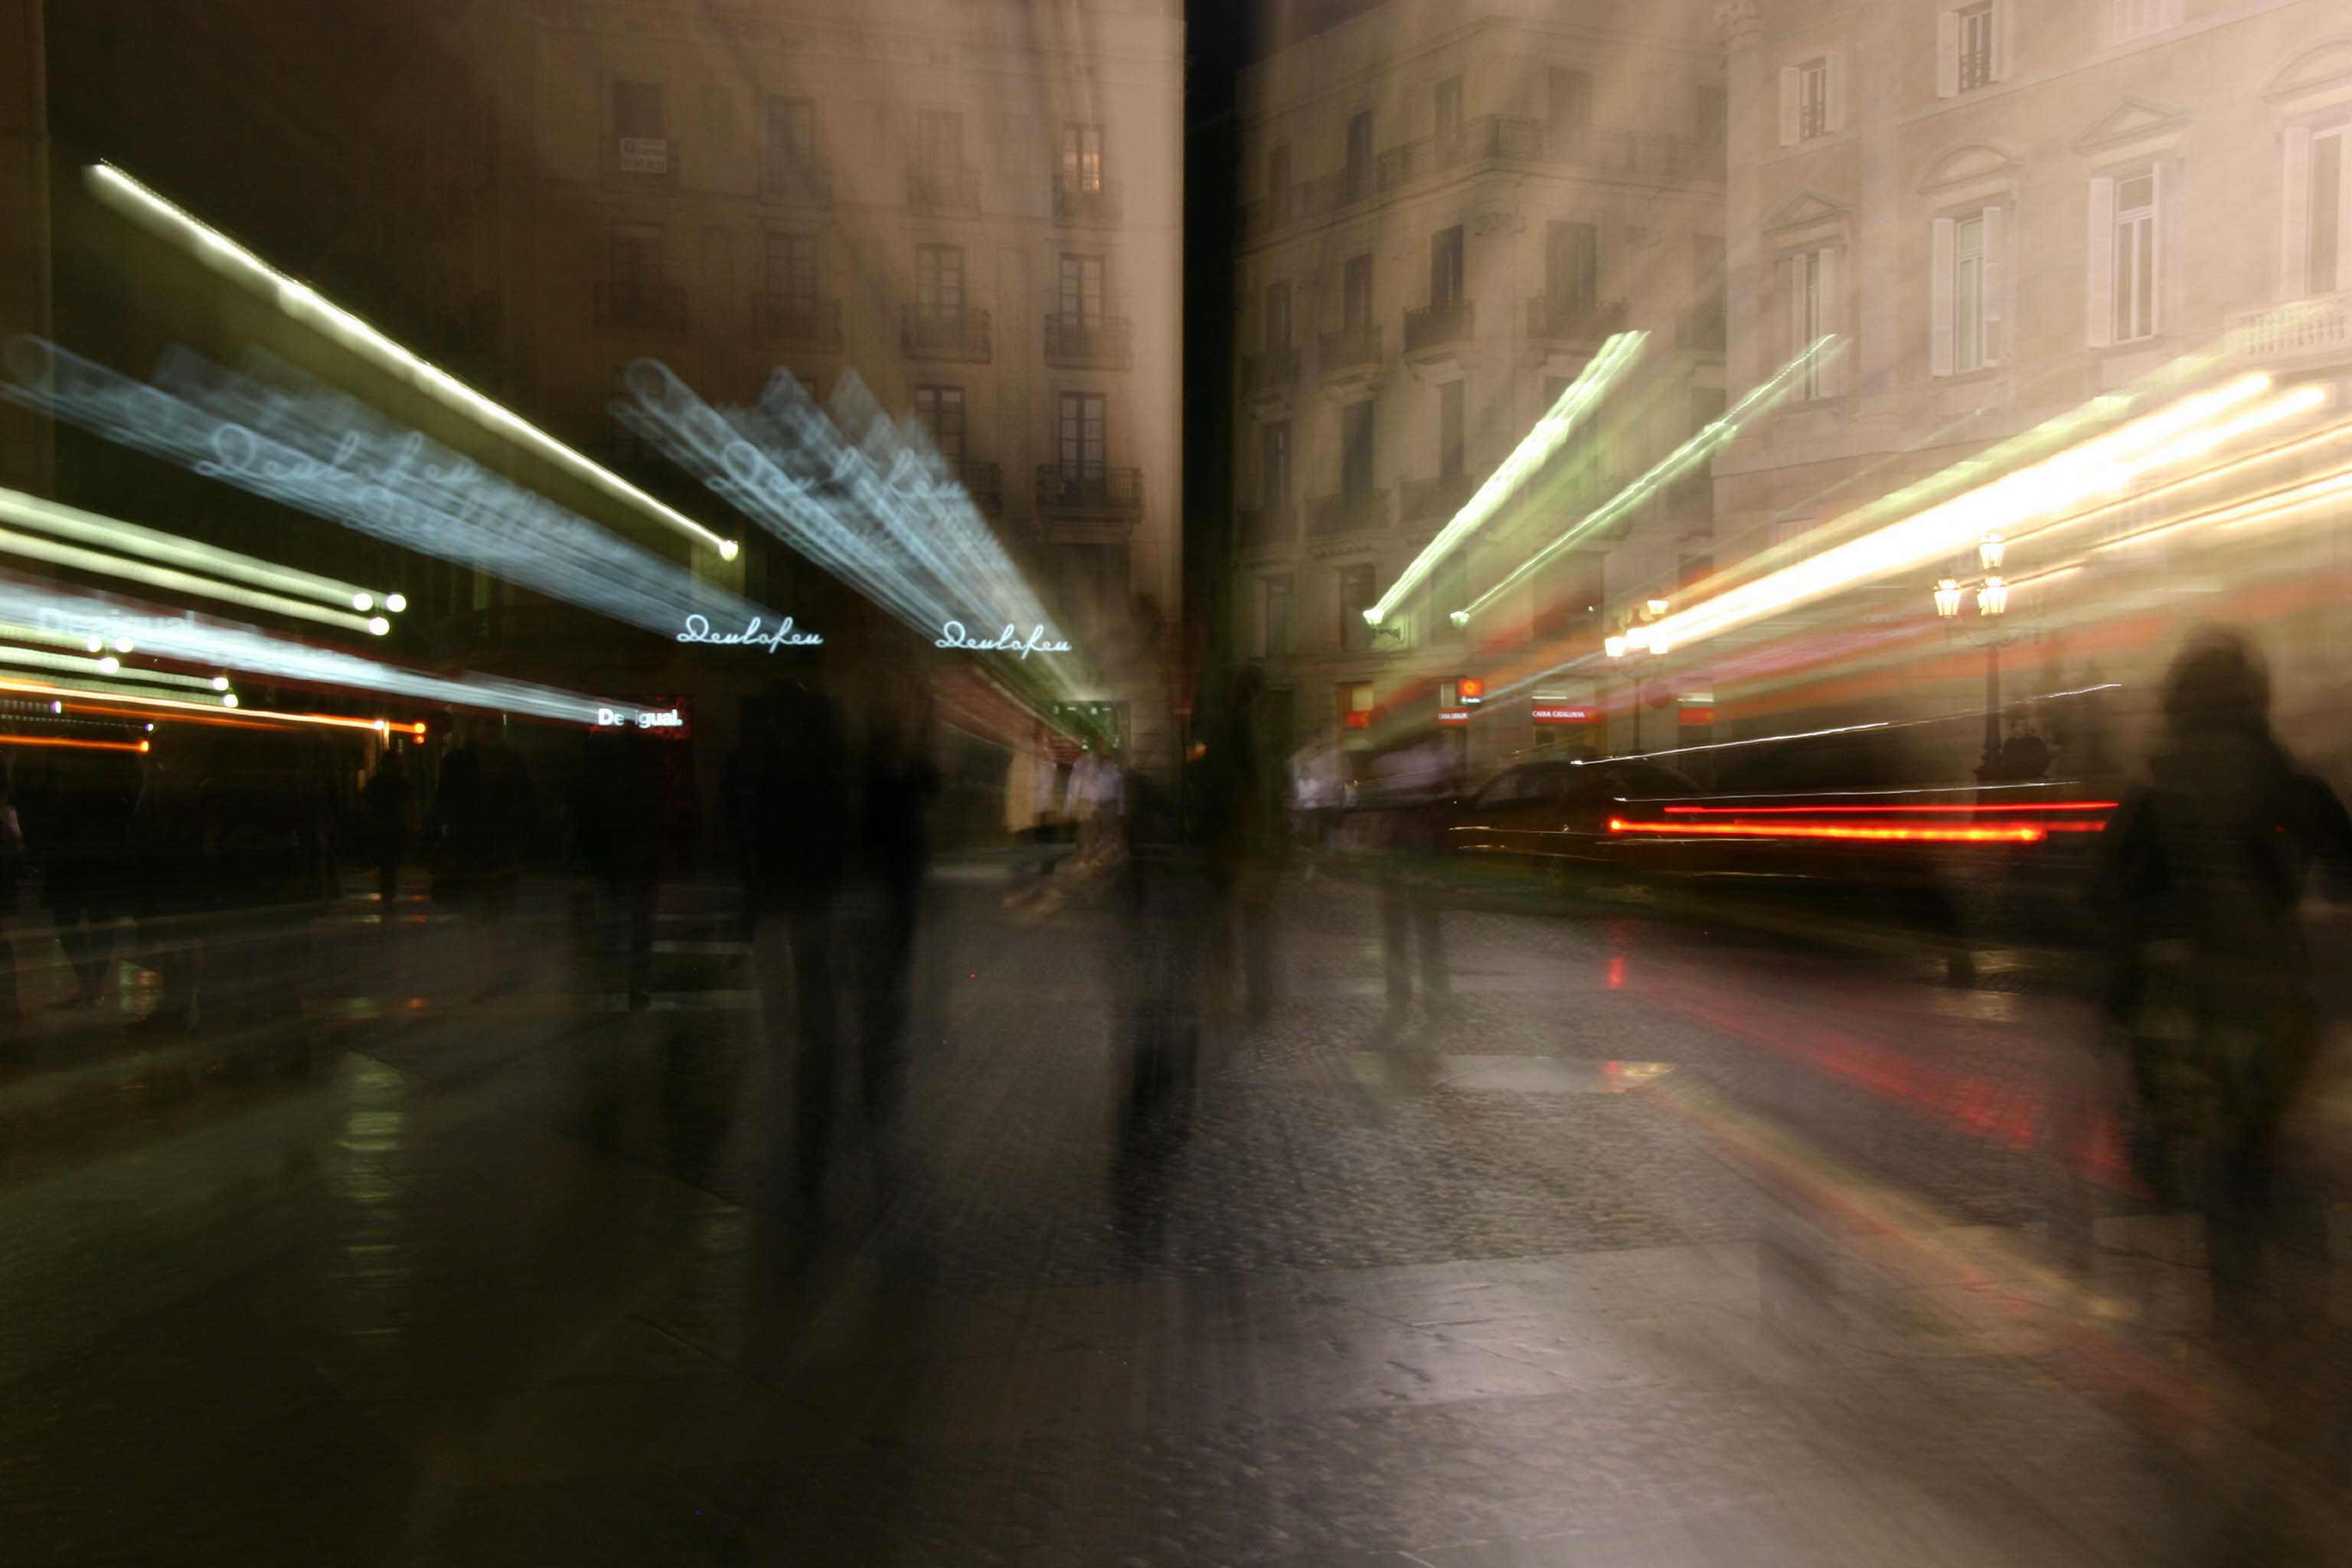
\includegraphics[height=\paperheight]{images/jaume_nit.jpg}
            };
            \node[fill=black, opacity=0, text opacity=1] at (5.5,-3.8) {\large{ \color{white} Getting Data from the Web with R}};
        \end{tikzpicture}
     \end{frame}
}

%------------------------------------------------

\begin{frame}[fragile]
\frametitle{Readme}

\begin{block}{\scriptsize License:}
\tiny
 \begin{itemize}
  \item[] Creative Commons Attribution-NonCommercial-ShareAlike 4.0 International License \\ 
  \url{http://creativecommons.org/licenses/by-nc-sa/4.0/}{}
 \end{itemize}
\end{block}

\begin{block}{\scriptsize You are free to:}
\tiny
 \begin{itemize}
  \item[] \textcolor{darkgray}{\textbf{Share}} --- \textcolor{gray}{copy and redistribute the material}
  \item[] \textcolor{darkgray}{\textbf{Adapt}} --- \textcolor{gray}{rebuild and transform the material}
 \end{itemize}
\end{block}

\vspace{2mm}
\begin{block}{\scriptsize Under the following conditions:}
\tiny
\begin{itemize}
 \item[] \textcolor{darkgray}{\textbf{Attribution}} --- \textcolor{gray}{You must give appropriate credit, provide a link to the license, and indicate if changes were made.}
 \item[] \textcolor{darkgray}{\textbf{NonCommercial}} --- \textcolor{gray}{You may not use this work for commercial purposes.}
 \item[] \textcolor{darkgray}{\textbf{Share Alike}} --- \textcolor{gray}{If you remix, transform, or build upon this 
 work, you must distribute your contributions under the same license to this one.}
\end{itemize}
\end{block}

\end{frame}

%------------------------------------------------

\begin{frame}
\frametitle{Lectures Menu}

\begin{columns}[t]
\begin{column}{0.1\textwidth}
%--- empty space ---%
\end{column}
\begin{column}{0.8\textwidth}
 \begin{block}{Slide Decks}
  \begin{enumerate}
   \item \textbf{Introduction}
   \item \textcolor{lightgray}{Reading files from the Web}
   \item \textcolor{lightgray}{Basics of XML and HTML}
   \item \textcolor{lightgray}{Parsing XML / HTML content}
   \item \textcolor{lightgray}{Handling JSON data}
   \item \textcolor{lightgray}{HTTP Basics and the RCurl Package}   
   \item \textcolor{lightgray}{Getting data via Web Forms}
   \item \textcolor{lightgray}{Getting data via Web APIs}
  \end{enumerate}
 \end{block}
\end{column}
\begin{column}{0.1\textwidth}
%--- empty space ---%
\end{column}
\end{columns}

\end{frame}

%------------------------------------------------

\begin{frame}
\frametitle{About these lectures}

\begin{columns}[t]
\begin{column}{0.1\textwidth}
%--- empty space ---%
\end{column}
\begin{column}{0.8\textwidth}
\begin{block}{Goal}
My goal is \textbf{to give you an introduction} to some of the tools in R for getting data from the Web.

\bigskip
I don't pretend to cover everything nor going very deep. I just want to show you an overview of various Web Data scenarios you can handle with R.
\end{block}
\end{column}
\begin{column}{0.1\textwidth}
%--- empty space ---%
\end{column}
\end{columns}

\end{frame}

%------------------------------------------------

\begin{frame}
 \begin{center}
  \Huge{\textcolor{mandarina}{Preliminaries}}
 \end{center}
\end{frame}

%------------------------------------------------

\begin{frame}
\frametitle{Requirements}

\begin{block}{Must have:}
 \begin{itemize}
  \item Some experience working with R
  \item Some knowledge of HTML
  \item An insatiable curiosity for learning new things
 \end{itemize}
\end{block}

\begin{block}{Nice to have:}
 \begin{itemize}
  \item Knowledge about data storage formats
  \item Some programming experience
  \item Knowledge on how the Web works
 \end{itemize}
\end{block}

\end{frame}

%------------------------------------------------

\begin{frame}
\frametitle{Software}

\begin{block}{You'll need:}
 \begin{itemize}
  \item R \textcolor{lightgray}{(preferably the last version)} \\ \url{http://cran.r-project.org/}
  \item RStudio \textcolor{lightgray}{(highly recommended)} \\ \url{https://www.rstudio.com/}
  \item Text Editor \\ \textcolor{lightgray}{(eg vim, emacs, TextWrangler, notepad, sublime text)}
  \item Web Browser \\ \textcolor{lightgray}{(eg Chrome, Safari, Firefox, Internet Explorer, Opera)}
  \item and a good internet connection!
 \end{itemize}
\end{block}

\end{frame}

%------------------------------------------------

\begin{frame}
\frametitle{In my case ...}

\begin{block}{Software I used for these slides:}
 \begin{itemize}
  \item R version 3.1.0 (2014-04-10) -- "Spring Dance"
  \item Platform: x86\_64-apple-darwin10.8.0 (64-bit)
  \item IDE: RStudio Version 0.98.501
  \item Text Editor: TextWrangler
  \item Web Browser: Google Chrome Version 34.0.1847.131
  \item Operating System: OS-X Version 10.8.5
 \end{itemize}
\end{block}

\end{frame}

%------------------------------------------------

\begin{frame}
\frametitle{Resources}

\begin{block}{Some R Books}
 \begin{itemize}
  \item XML and Web Technologies for Data Sciences with R \\ 
  \low{by Deb Nolan and Duncan Temple Lang}
  \item Introduction to Data Technologies \\ 
  \low{by Duncan Murdoch}
  \item Data Manipulation with R \\ 
  \low{by Phil Spector}
  \item more references in each slide deck
 \end{itemize}
\end{block}

\end{frame}

%------------------------------------------------

\begin{frame}
\frametitle{Resources}

\begin{block}{Web Scraping with R}
 \begin{itemize}
  \item Web scraping for the humanities and social sciences \\ 
  \low{(by Rolf Fredheim and Aiora Zabala)} \\
{\tiny \url{http://quantifyingmemory.blogspot.co.uk/2014/02/web-scraping-basics.html}}
  \item Web Scraping with R \low{(by Xian Nan)} \\
{\tiny \url{http://cos.name/wp-content/uploads/2013/05/Web-Scraping-with-R-XiaoNan.pdf}}
  \item R-bloggers posts on \textit{Web Scraping} \\ 
  {\tiny \url{http://www.r-bloggers.com/?s=web+scraping}}
 \end{itemize}
\end{block}

\end{frame}

%------------------------------------------------

\begin{frame}
\frametitle{Some R Packages}

\begin{center}
 \begin{tabular}{l l}
  \hline
  Package & Description \\
  \hline
  \highcode{RCurl} & R interface to the \code{libcurl} library \\
   & for making general HTTP requests \\
  \highcode{RHTMLForms} & Tools to process Web/HTML forms \\
  \highcode{XML} & Tools for parsing XML and HTML documents  \\
   & and working with structured data from the Web \\
  \highcode{RJSONIO} & Functions for handling JSON data \\
  \highcode{jsonlite} & Functions for handling JSON data \\
  \highcode{rjson} & Functions for handling JSON data \\
  \highcode{ROAuth} & Interface for authentication via OAuth 1.0 \\
  \highcode{SSOAP} & Use SOAP protocol to retrieve data \\
  \hline
 \end{tabular}
\end{center}

CRAN Task View: \textit{Web Technologies and Services} \\
 {\scriptsize \url{http://cran.r-project.org/web/views/WebTechnologies.html}}

\end{frame}

%------------------------------------------------

{ % all template changes are local to this group.
    \setbeamertemplate{navigation symbols}{}
    \begin{frame}[plain]
        \begin{tikzpicture}[remember picture,overlay]
            \node[at=(current page.center)] {
                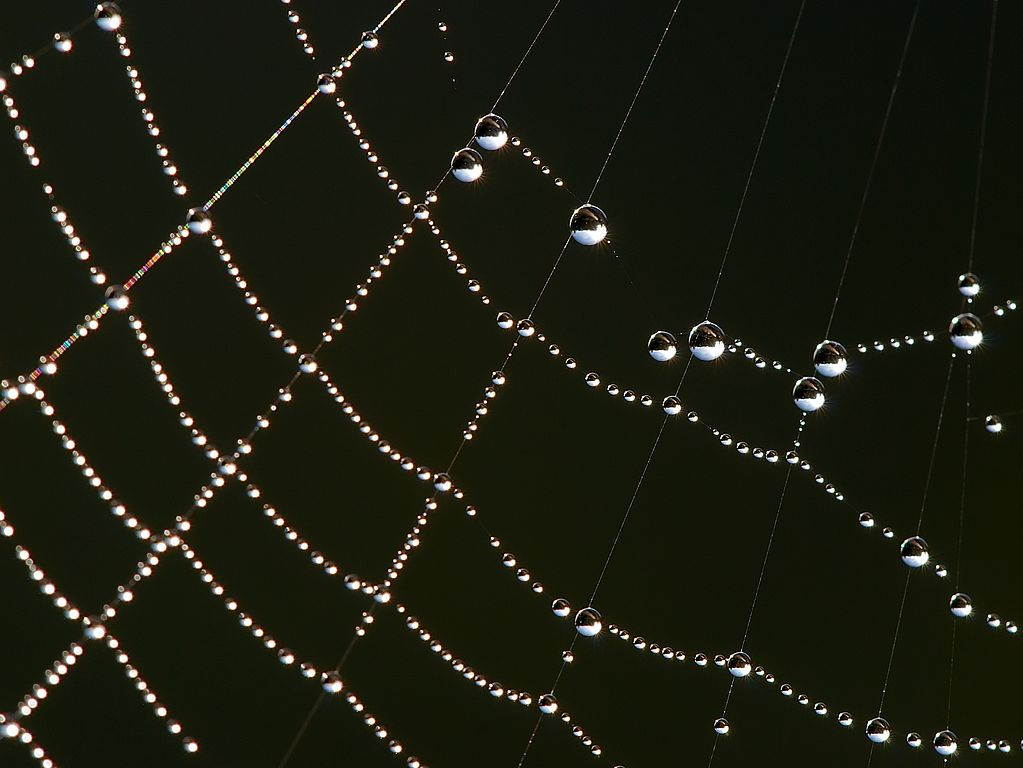
\includegraphics[width=\paperwidth]{images/spider_web.jpg}
            };
            \node[fill=black, opacity=0, text opacity=1] at (7.5,-2.8) {\Huge{ \color{white} The Web}};
        \end{tikzpicture}
     \end{frame}
}

%------------------------------------------------

\begin{frame}
\frametitle{VIP Questions}

\begin{columns}[t]
\begin{column}{0.1\textwidth}
%--- empty space ---%
\end{column}
\begin{column}{0.8\textwidth}
 \begin{block}{Very Important Preliminary Questions}
 The Data that you want:
 \begin{enumerate}
   \item Where is it located?
   \item How accessible is it?
   \item What is its structure / format? 
  \end{enumerate}
 \end{block}
\end{column}
\begin{column}{0.1\textwidth}
%--- empty space ---%
\end{column}
\end{columns}

\end{frame}

%------------------------------------------------

\begin{frame}
\frametitle{VIP Questions}

\begin{block}{Location of Data}
 \begin{itemize}
  \item Do you know the location (URL) beforehand?
  \item[] Or do you have to figure it out? \\
  \item Is it in one single specific place? \\
  \low{(eg one HTML table, one file in the Web)}
  \item Is it in one website but spread across several pages? \\
  \low{(eg several HTML tables at different pages)}
  \item Is it spread across several websites? \\
  \low{(eg multiple pieces of information in various sites)}
  \item Is it in one or several databases?
 \end{itemize}
\end{block}

\end{frame}

%------------------------------------------------

\begin{frame}
\frametitle{VIP Questions}

\begin{block}{Accessibility of Data}
 \begin{itemize}
  \item Do you have free direct immediate access to data?
  \item Do you need to fill a Web Form?
  \item Do you need to use a Web API?
  \item Do you require username, password, authentication?
  \item Do you need to use a specifc transfer protocol?
  \item Do you need to use a specifc type/method of request?
 \end{itemize}
\end{block}

\end{frame}


%------------------------------------------------

\begin{frame}
\frametitle{VIP Questions}

\begin{block}{Format / Structure of Data}
 \begin{itemize}
  \item Is it plain text? \\
  \item Is it in tabular \low{(spreadsheet-like)} form? \\
  \item Is it in HTML? \\
  \item Is it in some XML-dialect?
  \item Is it in JSON format?
  \item Other formats: binary, images, maps, etc?
 \end{itemize}
\end{block}

\end{frame}

%------------------------------------------------

\begin{frame}
\frametitle{Glossary}

\begin{block}{Some Acronyms}
 \begin{itemize}
  \item \textbf{WWW} World Wide Web
  \item \textbf{W3C} World Wide Web Consortium
  \item \textbf{URL} Uniform Resource Locator
  \item \textbf{HTTP} HyperText Transfer Protocol
  \item \textbf{XML} Extensible Markup Language
  \item \textbf{HTML} HyperText Markup Language
  \item \textbf{JSON} JavaScript Object Notation
 \end{itemize}
\end{block}

\end{frame}

%------------------------------------------------

\end{document}
